\documentclass[11pt]{article}

\usepackage{tikz}
\usepackage{amsmath}
\usepackage{amssymb}
\usepackage{amsthm}
\usepackage{relsize}
\usepackage{enumerate}
\usepackage{listings}

\title{Summary of important results}
\author{}
\date{}

\newcommand{\conj}[1]{\overline{#1}}
\newcommand{\sat}{\Vdash}
\newcommand{\cS}{\mathcal{S}}
\DeclareMathOperator{\gr}{gr}
\DeclareMathOperator{\Gr}{Gr}
\DeclareMathOperator{\val}{val}
\DeclareMathOperator{\col}{col}
\DeclareMathOperator{\fp}{fp}

\newcommand{\rightor}[3]{
\!\!\!
\mbox{
  \begin{tikzpicture}[baseline=-3pt]
    \draw[thick] (-1ex,0ex) node[left]{$#1\!$} -- (0ex,0ex);
    \draw[thick, ->] (0ex,0ex) -- (0.75ex,0.75ex) node[right]{\footnotesize $\!#2$};
    \draw[thick, ->] (0ex,0ex) -- (0.75ex,-0.75ex) node[right]{\footnotesize $\!#3$};
  \end{tikzpicture}
}
\!\!\!
}
\newcommand{\rightand}[3]{
\!\!\!
\mbox{
  \begin{tikzpicture}[baseline=-3pt]
    \draw[thick] (-0.75ex,0.75ex) node[left]{\footnotesize $#1$\!} -- (0,0);
    \draw[thick] (-0.75ex,-0.75ex) node[left]{\footnotesize $#2$\!} -- (0,0);
    \draw[thick, ->] (0,0) -- (1ex,0) node[right]{$\!#3$};
  \end{tikzpicture}
}
\!\!\!
}

\newcommand{\rightcurvearrow}{
\mathrel{
  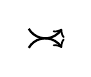
\begin{tikzpicture}[scale=0.8]
    \draw[thick,->] (0,1ex) arc (30:150:-2ex);
    \draw[thick,->] (0,-1ex) arc (150:30:2ex);
  \end{tikzpicture}
}
}
\newcommand{\rightcurveor}{
\!
\mathrel{
  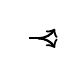
\begin{tikzpicture}[scale=0.8]
    \draw[thick,->] (0,0) arc (90:150:-2ex);
    \draw[thick,->] (0,0) arc (90:30:2ex);
    \draw[thick] (-1ex, 0) -- (0.1ex,0);
  \end{tikzpicture}
}\!
}
\newcommand{\Rightcurvearrow}{
\mathrel{
  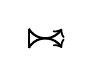
\begin{tikzpicture}[scale=0.8]
    \draw[thick,->] (0,1ex) arc (30:150:-2ex);
    \draw[thick,->] (0,-1ex) arc (150:30:2ex);
    \draw[thick] (0, 1ex) -- (0, -1ex);
  \end{tikzpicture}
}
}
\newcommand{\Rightcurveor}{
\mathrel{
  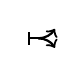
\begin{tikzpicture}[scale=0.8]
    \draw[thick,->] (0,0) arc (90:150:-2ex);
    \draw[thick,->] (0,0) arc (90:30:2ex);
    \draw[thick] (-1ex, 0) -- (0.1ex,0);
    \draw[thick] (-1ex, -0.7ex) -- (-1ex, 0.7ex);
  \end{tikzpicture}
}
}
\newcommand{\nRightcurvearrow}{
\mathrel{
  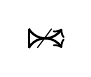
\begin{tikzpicture}[scale=0.8]
    \draw[thick,->] (0,1ex) arc (30:150:-2ex);
    \draw[thick,->] (0,-1ex) arc (150:30:2ex);
    \draw[thick] (0, 1ex) -- (0, -1ex);
    \draw (0.9ex, -1ex) -- (2.4ex, 1ex);
  \end{tikzpicture}
}
}
%todo mess with the symbols to make them look better


\newtheorem{prop}{Proposition}
\newtheorem*{prop*}{Proposition}
\newtheorem{corollary}{Corollary}
\newtheorem*{av}{Possible avenue of investigation}


\begin{document}

\maketitle

\tableofcontents

\section{Definitions}

\subsection{Propositional Logic}
%provisory telegraphic definitions. to be reviewed

We will work with a set $\Sigma$, which we will suppose finite for convenience, which will be our \emph{set of propositional symbols}.

A \emph{literal} is an element of $\Sigma \times \{\top, \bot\}$.

If $(a, v_a)$ is a literal, its \emph{conjugate}, denoted $\conj{(a,v_a)}$ is the literal $(a, \conj{v_a})$, where $\conj \top = \bot$ and $\conj \bot = \top$.

We say $\Gamma$ is a \emph{conjunctive normal form}, or \emph{CNF} if it is a set of \emph{clauses}. In turn, a clause is a set of literals.

We will, in general, obey the convention that a letter or literal is represented by a lower case letter, a clause by an upper case latin letter, and CNF by an upper case greek letter.

The clause $\{a,b,\cdots,z\}$ is usually denoted $a \vee b \vee \cdots \vee z$. In turn, the CNF $\{A, B, \cdots, Z\}$ is usually represented as $A \wedge B \wedge \cdots \wedge Z$.

A \emph{valuation on $\Sigma$} is a function from $\Sigma$ to $\{\top, \bot\}$.

Given a valuation $\rho$ and a literal $a = (\alpha, v_\alpha)$, we say $\rho$ satisfies $a$, denoted $\rho \sat a$ if and only if $\rho(\alpha) = v_\alpha$. Likewise, given a clause $C$ we say $\rho \sat C$ iff $\exists_{a \in C} \rho \sat a$. Finally, given a CNF $\Gamma$, we say $\rho \sat \Gamma$ iff $\forall_{C \in \Gamma} \rho \sat C$.

We will say a CNF $\Gamma$ is \emph{degenerate} if $\emptyset \in \Gamma$. These are not of interest, because any degenerate CNF is immediately not satisfiable.

\subsection{Logical symbols}

We want to do logical operations on $\top$ and $\bot$, such as ``or'', ``and'', implications, equivalence...

To distingish these operations from their ``meta'' versions, we will adopt the following conventions:

We will use $\vee$ and $\wedge$ as boolean operations, and for conjunction and disjunction we will resort to writing ``or'' and ``and''.

For boolean implication, we will use $\rightarrow$, reserving the symbol $\Rightarrow$ for meta-implication.

Finally, boolean equivalence is represented as $\leftrightarrow$, while meta-equivalence is represented by the usual $\Leftrightarrow$.


\subsection{Multigraphs}

A \emph{directed multigraph} $G$ is an ordered pair $(V, E)$ where $E$ is a set of \emph{multiedges} on V.

A multiedge on $V$ is an ordered pair $(A, B)$ where $A, B$ are subsets of $V$. This can be represented by the symbol $A \rightcurvearrow B$. We will often overload the term `edge' to mean multiedge, and the term `graph' to mean multigraph. When referring to graphs in the usual sense of the word (edges have one tail and one head), we will talk about `pure graphs'.

Informally, the edges on multigraphs represent implication in the following way: $A \rightcurvearrow B$ means ``If all elements of $A$ are true, then one element of $B$ must be true''. This motivates the following definition:

Fixed a multigraph $G = (V,E)$, we will work with colorations of the vertices with the colors $\top$ and $\bot$.

A coloration on $G$ is a function $\chi : V \rightarrow \{\top, \bot\}$.

Given a coloration $\chi$, we define:

\[ \chi \text{\emph{ is a valid coloration of $G$} iff } \forall_{(A,B) \in E} \left( \bigwedge_{\alpha \in A} \chi(\alpha) \rightarrow \bigvee_{\beta \in B} \chi(\beta) \right)\]

We will say that \emph{$A$ indirectly implies $B$}, denoted $A \Rightcurvearrow B$, if all valid colorings that color all of $A$ as $\top$ must cover one of $B$ as $\top$.

\subsection{Multigraphs from CNFs}

Given a CNF $\Gamma$, define the \emph{full graph of $\Gamma$}, denoted as $\Gr \Gamma$, as the graph $(V,E)$ such that $V$ is the set of literals, and

\[ E = \{ \, \conj A \rightcurveor (C \setminus A) \mid A \subseteq C, C \in \Gamma \, \}\]

Given a nondegenerate CNF $\Gamma$, define the \emph{tail graph of $\Gamma$}, denoted as $\gr \Gamma$, as the graph $(V,E)$ such that $V$ is the set of literals, and

\[ E = \{ \, \conj a \rightcurveor (C \setminus \{a\}) \mid a \in C, C \in \Gamma \, \}\]

Notice that this is a special kind of multigraph: one whose edges all have one and only one tail. We will call these \emph{tail graphs}.

Given a nondegenerate 2-CNF $\Gamma$, define the \emph{pure graph of $\Gamma$}, denoted as $\gr'\Gamma$, as the graph $(V,E)$ such that $V$ is the set of literals, and

\[ E = \{ \, \conj a \rightarrow b \mid \{a,b\} \in \Gamma \, \} \cup \{ \conj a \rightarrow a \mid \{a\} \in \Gamma \,\}\]

Notice this is a pure graph.

These three definitions have something in common: all of them somehow represent the CNF they originate from. We will make the meaning of this more precise:

We will assign to every multigraph $G = (V,E)$ (where $V$ is the set of literals) a unique CNF, which we will say is \emph{the CNF represented by $G$}. This is the CNF $\Gamma$ such that

\[\Gamma = \{\, \conj A \cup B \mid A \rightcurvearrow B \in E\,\}\]

As the reader may easily check, given a CNF $\Gamma$, it is the CNF represented by $\Gr \Gamma$, $\gr \Gamma$, and, if applicable, $\gr'\Gamma$. This will allow us to study some properties of all of these three at the same time.
\subsection{Valuations from colorings}

Given a set of propositional symbols $\Sigma$, we will deem a coloring $\chi$ of the literals with the colors $\top, \bot$ to be \emph{valorable} if, for all literals $v$, $\chi(\conj v) = \conj{\chi(v)}$.

\begin{prop}
To every valorable coloration $\chi$ one can correspond a unique valuation $\rho$ such that $\chi(a, \top) = \rho(a)$, and vice versa.

Define $\val \chi$ to be the valuation $\rho$ such that

\[\rho(\alpha) = \chi(\alpha, \top)\]

Likewise, define $\col \rho$ to be the valorable coloration $\chi$ such that

\[\chi(\alpha, v_\alpha) = \rho(\alpha) \leftrightarrow v_\alpha\]

The functions $\val$ and $\col$ are bijections from the valorable colorations to the valuations and vice versa.
\end{prop}

\begin{proof}
We will do this by showing they are each other's left and right inverse.

Let $\chi$ be a valorable coloration. Notice that

\[\col \val \chi (\alpha, v_\alpha) = \val \chi (\alpha) \leftrightarrow v_\alpha = \chi(\alpha, \top) \leftrightarrow v_\alpha\]

And a quick checking of both possible cases for $v_\alpha$ will show that this last thing equals $\chi(\alpha, v_\alpha)$.

On the other hand, let $\rho$ be a valoration. We have

\[\val \col \rho(\alpha) = \col \rho (\alpha, \top) = \rho(\alpha) \leftrightarrow \top = \rho(\alpha) \]

As we wished to show.
\end{proof}

The following propositions makes the bridge between satisfiability and validity.

\begin{prop}
If $\Gamma$ is represented by $G = (V,E)$ and $\rho$ is a valoration of $\Gamma$, $\chi = \col \rho$ is valid iff $\rho$ satisfies $\Gamma$.
\end{prop}

\begin{proof}
First, let us suppose $\rho$ is a colorating satisfying $\Gamma$. Consider the coloration of $G$ given by $\chi = \col \rho$. We wish to show it is valid.

To do this, pick any edge $\conj A \rightcurvearrow B$. By definition, we know $A \cup B \in \Gamma$, and as such, we know, since $\rho \sat \Gamma$, there either exists some $(\alpha, v_\alpha) \in A$ such that $\rho(\alpha) = v_\alpha$, or some $(\beta, v_\beta) \in B$ such that $\rho(\beta) = v_\beta$.

As such, either there exists some $a \in A$ such that $\chi(a) = \top$, or some $b \in B$ such that $\chi(b) = \top$, and thus, if $\chi$ was to color all elements of $\conj A$ as $\top$, it must color all elements of $A$ as $\bot$, and thus would color some element of $B$ as $\top$. In short: if $\chi$ colors all of $\conj A$ as $\top$, it must color some of $B$ as $\top$.

This shows $\chi$ is valid with relation to this particular edge, but since the choice was arbitrary, $\chi$ is valid with relation to all edges, and so $\chi$ is a valid coloration of $G$.

On the other hand, let us suppose that $\chi$ is valid. We will show $\rho$ satisfies $\Gamma$.

To do this, pick an arbitrary $C \in \Gamma$. By hypothesis, we know $C$ is of the form $A \cup B$, where $\conj A \rightcurvearrow B$ is an edge in $G$. Since $\chi$ is valid, we have that either it colors an element of $A$, or an element of $B$, as $\top$. As such for some $(\gamma, v_\gamma) \in C$ we have $\chi(\gamma, v_\gamma) = \top$, and so $\rho(\gamma)$ must equal $v_\gamma$, and so $\rho$ satisfies this literal, and thus this clause. Since the clause chosen was arbitrary, $\rho$ satisfies all clauses, and thus satisfies $\Gamma$.
\end{proof}

\begin{prop}
If $\Gamma$ is represented by $G = (V,E)$, then $\Gamma$ is satisfiable iff $G$ has a valid valorable coloration.
\end{prop}

\begin{proof}
Simply apply the previous proposition. If $\Gamma$ is satisfiable, pick a satisfying valuation and consider its coloration, which will be valid and valorable. If $G$ has a valid valorable coloration, consider its associated valuation.
\end{proof}

\subsection{Direct implication}

In the interest of characterizing the relation of indirect implication in the context of tail graphs, we will consider the following definition:

We define the relation \emph{$a$ n-implies $B$}, denoted as $a \rightcurveor_{\,n} B$, inductively as such:

\[\text{if } B = \{a\} \text{, then } a \rightcurveor_0 B\]


\[\text{if } a \rightcurveor_n B \text{, } b \in B \text{, and } b \rightcurveor C \text{, then } a \rightcurveor_{n+1} (B \setminus \{b\}) \cup B'\]

We say $a \rightcurveor_* B$ if there exists $n$ for which $a \rightcurveor_n B$.

This relation is a generalization of the idea ``there's a path from $a$ to $b$'' in pure graphs. In fact, if our graph is pure, $a \rightcurveor_* B$ if and only if $B$ is a singleton set $\{b\}$ and there is a path going from $a$ to $b$. $a \rightcurveor_n \{b\}$ if and only if there is a path of length $n$ from $a$ to $b$ in this case. This can easily be shown by induction.

\subsection{The exhaustion algorithm}

Consider an arbitrary multigraph $G = (V,E)$, and let $V_0 \subseteq V$

We will call the following the \emph{exhaustion algorithm}.

\begin{minipage}{\linewidth}
\begin{lstlisting}[mathescape]
$T \gets V_0$
$U \gets E$
While $\exists_{(A,B) \in U} \, A \subseteq T$:
    If $B = \emptyset$:
        Halt
    Else:
        Pick $v$ from $B$
        $T \gets T \cup \{v\}$
        $U \gets U \setminus \{(A,B)\}$
\end{lstlisting}
\end{minipage}

\section{Propositions}

\subsection{General results on multigraphs}

In the following, consider fixed a multigraph $G = (V,E)$.

\begin{prop}
The exhaustion algorithm halts, and when it does, if it has not halted prematurely, the coloration $\chi(a) = (\top \text{ if } a \in T \text{ else } \bot)$ is valid.
\end{prop}

\begin{proof}
To show that it halts, merely notice that the cardinality of $U$ decreases by 1 with each iteration.

To show that the coloration induced by $T$ is valid after it does, notice that whenever an edge $A \rightcurvearrow B$ is removed from $U$, you are sure to have at least one element of $B$ in $T$.

As such, we can split edges into two sets. Those that are still in $U$ don't have all of their tail elements painted $\top$, as if any did, that would lead to another run in the loop, and so they are valid. Those that are not in $U$ have at least one element of their head painted $\top$, and so they are valid.

As such, in the end, all edges are validated, and the coloring induced by $T$ is valid.
\end{proof}

\begin{prop}
If there is a valid coloration $\chi$ of $G$, starting the exhaustion algorithm with any subset of $S = \{ \, v \in V \mid \chi(v) = \top \, \}$, there is a sequence of choices that does not lead to premature halting.
\end{prop}

\begin{proof}
The idea is to take the greedy approach, and make sure $T$ is always a subset of  $S$.

Before the while loop, this is true by hypothesis. Every run of the while loop, an edge $A \rightcurvearrow B$ is chosen such that $A$ is contained in $T$, and thus, in $S$. Therefore, some element of $B$ is contained in $S$. Pick that element. The condition that $T \subseteq S$ remains true, which preserves our invariant, allowing for yet another run of the loop, and so on until termination.
\end{proof}

It will be useful to study all the possible outputs of the exhaustion algorithm, and as such, we make the following definition:

A \emph{state} is a pair $\cS = (T,U)$, where $T \subseteq V$ and $U \subseteq E$. The set of \emph{successors of a state $\cS = (T,U)$}, denoted $s(\cS)$, is defined as follows:

If there exists no $(A,B) \in U$ such that $A \subseteq T$, define $s(\cS)$ as $\{(T, \emptyset)\}$.

Otherwise, define $s(\cS)$ as

\[ \{ \, (T \cup \{v\}, U \setminus \{(A,B)\}) \mid (A,B) \in U, A \subseteq T, v \in B \, \}\]

It is easy to recognize $s(\cS)$ as ``the set of states we can be in after one iteration of the exhaustion algorithm, bar premature halting''.

Define $\cS^n$ inductively as: $\cS^0 = \{\cS\}$, $\cS^{n+1} = \cup_{R \in \cS^n} s(R)$. In other words, ``the set of states we can be in after $n$ iterations of the exhaustion algorithm, bar premature halting''.

The previous results can be mirrored as results about states.

\begin{prop}
Fixed a state $\cS = (T_0, U_0)$, there exists $n$ such that $\cS^{n+1} = \cS^n$.

We will refer to this `fixed point' as $\fp \cS$.

Given a graph $G = (V,E)$, suppose we start with $T_0 \subseteq V$, $U = E$. Fixed any state $(T,U)$ in the fixed point, the coloration of $G$ induced by $T$ is valid.
\end{prop}

\begin{proof}
To show the fixed point exists, consider the families $U^n = \{\,U\mid (T,U) \in \cS^n\,\}$. Consider the maximum cardinality of the elements of $U^n$.

For $n = 0$, this maximum cardinality is clearly $\# U_0$. Now, notice that this maximum cardinality always decreases, unless it is zero. When this max cardinality is zero, we are in a fixed point.

To show that, for all $(T,U) \in \fp \cS$, the coloration induced by $T$ is valid, merely notice that, for all $n$, all states of $\cS^n$ obey the following property: if $A \rightcurvearrow B$ is not in $U$, then either there exists some element of $B$ in $T$, or there exists an element of $A$ not in $T$. This is easy to see in virtue of how the elements are removed from $U$.

As such, since at the end, all states have $U$ empty, all edges are valid with respect to their respective $T$, and so the colorations are valid.

%This is pretty piss poorly written. Find a better way to do this.
\end{proof}

\subsection{Full graphs}

\begin{prop}
Let $\Gamma$ be a CNF, ${A \rightcurvearrow B}$ an edge of $\Gr \Gamma$.

$A$ and $\conj B$ are disjoint.
\end{prop}

\begin{prop} (Symmetry)
Under the same assumptions, if ${a \in A}$, then ${(A \setminus \{a\}) \rightcurvearrow (B \cup \{\conj a \})}$ is an edge. Likewise, if ${b \in B}$, then ${(A \cup \{\conj b\}) \rightcurvearrow (B \setminus \{b\})}$ is as well.
\end{prop}

To word the latter differently:

\begin{prop*}
If $a \not\in A$ and $\conj a \not\in B$, then $(A \cup \{a\}) \rightcurvearrow B$ iff $A \rightcurvearrow (B \cup \{\conj a\})$.
\end{prop*}

\begin{prop}
If $\chi$ is a valid coloration of a graph $G$, its restriction to $V \setminus \{a\}$ is a valid coloration of $G_{\setminus a}$.
\end{prop}

\begin{prop}
Let $\Gamma$ be a CNF, $G$ its graph, and suppose $\chi$ is a valid coloration of $G_{\setminus a}$. Then, it can be extended to a valid coloration of $G$ by putting $\chi(a) = \conj{\chi(\conj a)}$.
\end{prop}

\begin{corollary} \label{swapvalue}
If $\chi$ is a valid coloration of $G$, fixed $a \in V$, the coloration obtained from $\chi$ by changing $\chi(a)$ to $\conj{\chi(\conj a)}$ is valid.
\end{corollary}

\begin{prop}
Let $\Gamma$ be a CNF, $G$ its corresponding graph.

$\Gamma$ is satisfiable iff there exists a valid coloration of $G$.
\end{prop}

\begin{corollary}
$\Gamma$ is not satisfiable iff $\emptyset \Rightcurvearrow \emptyset$.
\end{corollary}

\begin{prop}
Fixed an arbitrary multigraph $G$, indirect implication in this graph has the following three properties:

\begin{enumerate}[i]
\item If $A \rightcurvearrow B$, then $A \Rightcurvearrow B$
\item (Extensionality) If $A' \supseteq A$, $B \subseteq B'$, and $A \Rightcurvearrow B$, then $A' \Rightcurvearrow B'$.
\item (Concatenation) If $A \Rightcurvearrow \{x\}$ and $\{x\} \Rightcurvearrow B$, then $A \Rightcurvearrow B$.
\end{enumerate}
\end{prop}

\begin{av}
Is there a complete calculus for finding indirect implication, based on the above rules and perhaps some more?
\end{av}

\begin{prop} (Symmetry)
In the context of the full graph of a CNF:

If $\conj a \not \in A$ and $a \not \in B$, then

\[ A \cup \{a\} \Rightcurvearrow B \text{ iff } A \Rightcurvearrow B \cup \{\conj a\} \]
\end{prop}

An important detail to take note of: while the symmetry for direct and indirect implication is very similar, there is a subtle but important difference: in direct implication, we must assume $a \not \in A \cup \conj B$. Here we assume exactly the opposite: $\conj a \not \in A \cup \conj B$.

\begin{prop}
Let $\Gamma$ be a CNF formula, $G = (V, E)$ its full graph.

Run the exhaustion algorithm with $V_0 = \emptyset$.

$\Gamma$ is satisfiable iff there is a sequence of choices that lead to this algorithm not halting prematurely.

If such a thing happens, the valuation $\rho(\alpha) = \top \text{ if } (\alpha, \top) \in T \text { else } \bot$ satisfies $\Gamma$.
\end{prop}

\subsection{Tail graphs}

\begin{prop}
Let $\Gamma$ be a CNF.

Furthermore, let $\rho$ be a valuation of $\Sigma$, and $\chi = \col \rho$.

Then, $\rho \sat \Gamma$ iff $\chi$ is valid on $\gr \Gamma$.
\end{prop}

\begin{corollary}
$\Gamma$ is satisfiable iff there exists a valid valorable coloration of its tail graph.
\end{corollary}

I'm sure I'll find more stuff to put here.

The following is possibly the best result I've got here.

\begin{prop}
Let $G = (V,E)$ be a tail graph.

$a \Rightcurveor B$ iff there exists a subset $B'$ of $B$ such that $a \rightcurveor_* B'$.

This is proven by showing that they are both equivalent to:

There exists no state $(T,U)$ in $\fp (\{a\}, E)$ such that $T$ is disjoint from $B$.
\end{prop}

\begin{av}
Try to broaden this to non-tail graphs.
\end{av}

\subsubsection{2-CNF}

\begin{prop}
Let $\Gamma$ be a 2-CNF, $V$ the literals.

A valorable coloration of $V$ is valid in $\gr \Gamma$ iff it is valid in $\gr' \Gamma$.
\end{prop}

(A bunch of auxiliary results will probably end up being here...)

This is the main objective of this project: the main result of \cite{2cnf}, proven with a different approach.

\begin{prop}
Let $\Gamma$ be a 2-CNF.

$\Gamma$ is satisfiable iff there is no cycle in $\gr' \Gamma$ that passes through a vertex and its conjugate at the same time.
\end{prop}


\begin{thebibliography}{1}

\bibitem{2cnf}
\textit{A linear-time algorithm for testing the truth of certain quantified boolean formulas}

\end{thebibliography}
\end{document}
